\documentclass[oupdraft]{bio}
\usepackage[colorlinks=true, urlcolor=citecolor, linkcolor=citecolor, citecolor=citecolor]{hyperref}

% Add history information for the article if required
\history{Received August 1, 2010;
    revised October 1, 2010;
accepted for publication November 1, 2010}

\begin{document}

% Title of paper
\title{Overcoming confounding plate effects in differential expression analyses of single-cell RNA-seq data}

% List of authors, with corresponding author marked by asterisk
\author{AARON T. L. LUN$^{1,\ast}$, JOHN C. MARIONI$^{1,2,\ast}$ \\[4pt]
    % Author addresses
    \textit{$^1$Cancer Research UK Cambridge Institute, University of Cambridge, Li Ka Shing Centre, Robinson Way, Cambridge CB2 0RE, United Kingdom;
$^2$EMBL European Bioinformatics Institute, Wellcome Genome Campus, Hinxton, Cambridge CB10 1SD, United Kingdom}
    \\[2pt]
    % E-mail address for correspondence
{aaron.lun@cruk.cam.ac.uk, marioni@ebi.ac.uk}}

% Running headers of paper:
\markboth%
% First field is the short list of authors
{A. T. L. Lun and J. C. Marioni}
% Second field is the short title of the paper
{Overcoming plate effects in DE analyses of scRNA-seq data}

\maketitle

% Add a footnote for the corresponding author if one has been
% identified in the author list
\footnotetext{To whom correspondence should be addressed.}

\begin{abstract}{
An increasing number of studies are using single-cell RNA-sequencing (scRNA-seq) to characterize the gene expression profiles of individual cells.
One common analysis applied to scRNA-seq data involves detecting differentially expressed (DE) genes between cells in different biological groups.
However, many experiments are designed such that the cells to be compared are processed in separate plates or chips, 
    meaning that the groupings are confounded with systematic plate effects.
This confounding aspect is frequently ignored in DE analyses of scRNA-seq data.
In this article, we demonstrate that failing to consider plate effects in the statistical model will result in loss of type I error control.
A solution is proposed whereby counts are summed from all cells in each plate, and the count sums across all plates are used in the DE analysis.
This restores type I error control in the presence of plate effects without compromising detection power in simulated data.
The summation approach is also robust to varying numbers and sizes of cells per plate.
Similar results are observed in DE analyses of real data where the use of count sums and single-cell counts lead to a different number and ranking of DE genes.
This suggests that summation can help in maintaining statistical rigour in DE analyses of scRNA-seq data with plate effects.
}
{Single-cell RNA sequencing; Differential expression; Plate effects; Summation.}
\end{abstract}


% Supplementary sections
\newcommand{\suppimplementation}{1}
\newcommand{\suppquantile}{2}
\newcommand{\suppmeanvar}{3}
\newcommand{\suppnorm}{4}

% Supplementary figures
\newcommand{\suppcompsim}{S1}
\newcommand{\suppexpprof}{S2}

\section{Introduction}
Single-cell RNA sequencing (scRNA-seq) is increasingly being used to study molecular biology at the cellular level.
RNA is isolated from individual cells and reverse-transcribed into cDNA fragments that are sequenced using massively parallel technologies \citep{stegle2015computational}.
Mapping of the sequence reads to a reference genome allows quantification of gene expression in each cell based on the number of reads assigned to each gene.
The count data can then be analyzed to identify cell subtypes by clustering of the gene expression profiles;
    to identify highly variable genes contributing to cell-to-cell heterogeneity;
    and to identify differentially expressed (DE) genes between groups of cells.
The ability to assay expression profiles for individual cells provides scRNA-seq studies with biological resolution that cannot be matched by bulk RNA-seq experiments on cell populations.
However, this comes at the cost of high technical noise due to the difficulties in sequencing low input quantities of RNA from single cells.

Most existing scRNA-seq protocols are based either on microwell plates \citep{picelli2014full} or microfluidics systems like the Fluidigm C1 \citep{pollen2014low}.
In the former, cells are placed into individual wells, typically with automated approaches such as fluorescently activated cell sorting (FACS).
The entire plate is processed to generate sequencing libraries for all cells at once.
In the latter, individual cells are captured in separate reaction chambers within the C1 chip 
    (for simplicity, each chip will be treated as being equivalent to a plate in the following text).
All cells on each chip are then simultaneously processed into libraries.
Each plate or chip can only handle a limited number of cells, so data are usually generated for multiple plates across several biological groups. 
All cells on each plate typically come from the same population (e.g., culture, embryo, animal) of a single biological group.
If replicate populations are present in a group, a separate plate is used for cells from each population.

The experimental design described above is motivated largely by practicality.
It is logistically simpler to track and process cells when each plate corresponds to one population of one group, compared to partitioning the plate into different groups.
For example, FACS is typically performed such that all cells on a plate are derived from the same gates, i.e., from the same subpopulation.
In the C1, cells are captured randomly in reaction chambers such that the identity of the cell in each chamber cannot be pre-specified.
Ambiguity in determining the group for each cell is avoided by only using cells from the same group on each chip.
However, this design can result in a ``plate effect'' where uncontrollable experimental variables have a consistent effect for all cells on each plate but a variable effect across different plates. 
These variables can be technical in origin, such as differences in library preparation or sequencing efficiency between plates; 
    or biological, due to inherent variability in gene expression across replicate populations on different plates.

% Yeah, yeah, indexed FACS, I know. But there's a lot of experimental designs that don't use that.

One common analysis applied to scRNA-seq data involves identifying DE genes between groups of cells.
This does not strictly require single-cell resolution, and is more conventionally performed with bulk data.
Nonetheless, there are some benefits to using single-cell data in this context.
Rare cells are more easily sequenced with single-cell protocols, and irrelevant cells from contaminating populations can be screened out before analysis.
It is also more practical to perform the DE analysis on existing scRNA-seq data compared to generating bulk data exclusively for this purpose.
The DE analysis itself is typically performed using methods such as edgeR \citep{robinson2010edgeR} and DESeq \citep{anders2010differential}, which were designed for bulk data;
    or with methods such as Monocle \citep{trapnell2014dynamics} and SCDE \citep{kharchenko2014bayesian}, which were designed explicitly for single-cell data.
Putative DE genes are defined as those that exhibit significant differences in the average counts between two or more groups of interest.

The presence of plate effects complicates the parametrization of the experimental design in the DE analysis.
Obviously, such effects are undesirable as they arise via uncontrolled experimental variability.
This increases the estimated variance and reduces the power to detect DE genes.
However, they cannot be easily removed during the statistical modelling, since the plate effect is confounded with the groups of interest \citep{hicks2015widespread}.
At the most extreme, consider a data set with multiple groups where each group is comprised of cells from a single plate.
Changes in gene expression due to a plate-specific effect will be indistinguishable from genuine DE between groups.
Any attempt to remove the former will compromise the detection of the latter.
This problem is still present in data sets with small numbers (e.g., 2-3) of plates in each group, 
    where stochastic plate-to-plate variability may explain some or all of the apparent DE between groups.
In the absence of a suitable method to remove plate effects, most studies have simply ignored them and treated cells from different plates as direct replicates \citep{kolod2015single,trapnell2014dynamics,avraham2015pathogen}.
This strategy may not be statistically rigorous as the variability across cells will not be modelled properly.

This article demonstrates that plate effects must be handled appropriately to maintain the statistical validity of a DE analysis.
In a simple simulation, all analyses that ignored the plate effects failed to control the type I error rate.
This was caused by dependencies between cells on the same plate, which compromised inferences from the fitted model.
To avoid detection of spurious DE, a summation approach is proposed whereby counts for all cells on each plate were summed prior to the DE analysis.
This restored control of type I error across a range of simulation scenarios, without compromising DE detection power.
Similar effects were observed in real data where summation resulted in substantial changes in the number and ranking of DE genes.

\section{Plate effects result in false positives in a DE analysis}

\subsection{Description of the experimental design and analysis strategies}
Consider an experimental design consisting of multiple biological groups of interest.
Each group consists of cells sorted onto multiple plates, where all cells on each plate come from an independent population of a single group.
As previously mentioned, this is not an uncommon setup due to the logistics of the experimental protocol, e.g., cell sorting onto a plate with FACS, cell capture with the C1.
Further assume that a plate effect exists in the data set, whereby the expression of each gene in all cells of a given plate is modified in a gene- and plate-specific manner.
This setup is motivated by biological variability between replicate populations.
Stochastic differences in population-wide expression for each gene will result in gene-specific population-wide (and thus, plate-wide) effects on the expression of that gene for all constituent cells of each population.
Now, let the observed read count for gene $i$ in cell $j$ in plate $k$ of group $g$ be distributed as 
\[
    y_{ij} | \delta_{ik}  \sim X_{ik}
\]
where $\delta_{ik}$ is the plate-specific effect for this gene.
$X_{ik}$ is some random variable such that 
\[
    E(X_{ik}) = \lambda_{ik} = \delta_{ik}\mu_{ig}
\]
where $\mu_{ig}$ is the expected read count for group $g$. 
Any references to the conditional distribution, variance or mean will refer to the corresponding attributes of $X_{ik}$.
The plate effect $\delta_{ik}$ is sampled from some independent distribution $Z$ where $E(Z) = 1$, which ensures that $E(y_{ij}) = \mu_{ig}$.

% Obviously, you do get stochastic population-wide differences, e.g., due to culture conditions affecting all cells of a population in a gene-specific manner.
% Otherwise, if you didn't, it would all cancel out for millions of cells and bulk RNA-seq would have Poisson-level variability.

One aim of the data analysis for this experiment is to identify DE genes between groups.
However, this is complicated by the presence of the plate effects.
These effects cannot be removed by scaling normalization, e.g., based on library size or with more sophisticated methods \citep{anders2010differential,robinson2010scaling}.
This is because the plate effect varies for each gene, whereas the scaling factor for normalization of each cell is constant across genes.
The plate effects are also confounded by the biological group, as previously described.
A fold-increase in $\delta_{ik}$ cannot be distinguished from a matching increase in $\mu_{ig}$, based solely on the counts for a single plate.
Any attempt to remove the former will affect detection of genuine DE in the latter.
Even with multiple plates per group, this problem is still present as stochastic increases in $\delta_{ik}$ for all plates in a group can explain part or all of the observed DE between groups.

A common strategy ignores the plate effects and treats the cells from different plates as direct replicates.
The estimated variance will include the conditional variance between cells on a given plate, i.e., var$(X_{ik})$, as well as the variance of $\delta_{ik}$ between plates.
Methods can then be applied to detect DE between groups, using software designed for bulk RNA-seq data (e.g., DESeq) or with dedicated single-cell methods (e.g., Monocle).
This approach has been used in a number of scRNA-seq studies to detect DE across plates or chips \citep{kolod2015single,trapnell2014dynamics,avraham2015pathogen}.
However, it is not clear whether statistical rigour is maintained when plate effects are unaccounted for.

% Trapnell paper uses one C1 chip for each timepoint.
% Kolod...'s paper has multiple chip for each serum condition.
% Avraham's paper has 192 cells for the Salmonella exposed, and 96 for unexposed; this must be different plates.

\subsection{Simulating plate effects to evaluate analysis methods}
A simple simulation is used to test the performance of the analysis when plate effects are ignored.
Let the count for each gene in each cell follow a negative binomial (NB) distribution, conditional on the plate effect.
In other words, $X_{ik}$ represents a NB-distributed random variable with a mean of $\delta_{ik}\mu_{ig}$ and a dispersion of $\varphi_{i}$.
The size of $\varphi_{i}$ determines the variance of the conditional distribution and represents the magnitude of the cell-to-cell heterogeneity within each plate.
The plate effects themselves are sampled from a log-normal distribution, i.e., $Z \sim \ln \mathcal{N}(-\sigma^2/2, \sigma^2)$.
This parametrization ensures that $E(Z)=1$, as originally defined.

Simulated data were generated for 10000 genes across two groups, where each group consisted of three replicate plates with 50 cells in each plate.
The expected read count for each group was set to $\mu_{ig}=\mu_{i0}$ to simulate non-DE genes.
The value of $\mu_{i0}$ was sampled from $\exp(A)$ where $A \sim \mbox{Uniform}(3, 8)$, to recapitulate the spread of abundances for different genes in real data. 
For each gene $i$, the NB dispersion was defined according to the mean, i.e., 
\[
    \varphi_{i} = \frac{1}{2} + \frac{100}{\mu_{i0}} 
\]
to represent the decreasing mean-dispersion trend observed in real data.
The constants in the above expression were chosen to yield large values of $\varphi_{i}$, consistent with high technical and biological variability in scRNA-seq counts.
Finally, $\sigma^2$ was set to a value of 0.5 to generate a strong plate effect.
Simulations were repeated with $\sigma^2=0$ (i.e., no plate effect) as a control. 

These simulations use the same dispersion across all plates for each gene, rather than using plate-specific values.
This is done to fulfill the distributional assumptions of methods like edgeR and DESeq, which do not accommodate variable dispersions between counts for the same gene.
The use of a constant dispersion across counts simplifies the interpretation of the results by precluding variability in the dispersions as a cause for any poor performance of these methods.

\subsection{Implementation of DE analysis methods}
DE analyses of the simulated data were performed using edgeR, DESeq2 \citep{love2014moderated}, voom \citep{law2014voom}, Monocle and MAST \citep{finak2015mast}.
edgeR, DESeq2 and voom are methods designed for analyses of bulk RNA-seq data.
edgeR and DESeq2 model counts with NB distributions, while voom uses a normal distribution to model log-counts per million (log-CPMs) with precision weights.
Monocle and MAST were explicitly designed for analyzing scRNA-seq data, and operate on pre-processed expression values such as (log-)CPMs.

Each method was applied on the simulated data to test for DE between groups. 
In all methods, the experimental design was parametrized as a one-way layout with two groups.
All cells within each group were treated as direct replicates -- the plate of origin within each group was ignored.
edgeR was run twice, using either the quasi-likelihood (QL) framework \citep{lund2012detecting} 
    or using the likelihood ratio test (LRT) \citep{mccarthy2012differential} without empirical Bayes (EB) shrinkage of the NB dispersions.
Similarly, voom was run once with the one-way layout, and again after estimating the correlations induced by the plate effect.
The implementation details for each method are described in Section~\suppimplementation{} of the Supplementary Materials.

In all analyses, the null hypothesis is true for each gene $i$ as $\mu_{ig}$ is constant for all $g$.
Any rejections of the null represent type I errors, i.e., false positives.
For a specified type I error rate $\alpha = 0.01$, the observed error rate was defined as the proportion of all genes with a $p$-value below $\alpha$.
This was averaged across 10 simulation iterations to obtain a stable estimate of the observed type I error rate for each method. 
A method was considered to be liberal if its observed error rate in the simulation was above the specified $\alpha$.
Note that this evaluation is only possible for methods that compute $p$-values for each gene -- 
    Bayesian methods \citep{kharchenko2014bayesian} are not directly comparable as they generate posterior probabilities, and so are not tested here.

% BASiCS requires spike-ins, that the other methods don't use, so it's not entirely comparable.
% Kharchenko's method generates z-scores and MLEs, but no p-values.

\subsection{Type I error control is lost by all methods}
The observed type I error rate exceeds the specified threshold in all methods (Figure~\ref{fig:platefail}).
For all methods except for voom with correlations, the discrepancy between the observed and specified rates is greater than an order of magnitude.
This liberalness is attributable to the plate effect, rather than any inherent fault with the methods.
In the control simulation with $\sigma^2=0$, the observed rates for all methods are substantially closer to the threshold, if not below it.
These results suggest that DE analyses will perform poorly if the plate effect is simply ignored.
Loss of type I error control will result in an unacceptable number of false positives in the final set of DE genes.
This is equally applicable to the false discovery rate (FDR), given that control of the FDR depends on proper control of the type I error when the null hypothesis is true.

Loss of error control is caused by ignoring the plate effects in the statistical model.
In the one-way layout, the count of each gene in each cell is modelled by a distribution with a group-specific mean.
Most DE analysis methods assume that the counts for all cells are independently sampled from these distributions.
However, this is not the case when a plate effect is present.
The true mean of the sampling distribution for each cell is scaled by a plate-specific factor, 
    such that the counts for cells on the same plate are more similar than expected under independence.
(Conditional independence is irrelevant here, as the plate of origin is not used in the model parametrization.)
This reduces the amount of information in the data set as cells on the same plate are effectively redundant.
Methods that assume independence will overstate the information available to estimate model parameters such as the group-specific means, the variance or the NB dispersion.
This results in overconfident inferences and liberalness during hypothesis testing.

The problem can also be described in terms of the residual degrees of freedom (d.f.) that are available in the fitted model.
The simulation uses an experimental design with $6 \times 50 =  300$ cells and two coefficients in a one-way layout.
If all cells were truly independent -- as is assumed by most methods -- this design would provide 298 residual d.f. 
At the other extreme, consider the scenario where all cells on a plate have identical counts, i.e., there is no noise or heterogeneity between cells.
This means that there are only six independent samples (one cell per plate, as all other cells on that plate are redundant) and only four residual d.f.
This is substantially smaller than the expected 298 d.f., meaning that the uncertainty of various parameter estimates will be underestimated.
For example, the use of edgeR with the LRT assumes that sufficient residual d.f.\ are present to estimate the dispersion for each gene separately,
    without requiring EB shrinkage to share information between genes.
This is no longer justifiable if only four d.f.\ are available.

It is worth pointing out that voom with correlations explicitly accounts for the dependencies between cells.
This method exhibits the best performance of all tested methods in the presence of a plate effect (Figure~\ref{fig:platefail}),
    i.e., the observed type I error rate is closest to the specified threshold.
Nonetheless, voom with correlations is still liberal.
This is attributable to the difficulties in accurately estimating the consensus correlation when the number of plates is low.
In particular, underestimation will result in loss of type I error control as the dependencies will not be fully modelled.
This may also be compounded by the inadequacy of the normal model for highly discrete counts, particularly in scRNA-seq where low-abundance genes have many zero counts.

% Discreteness is secondary, as voom itself does fine without a plate effect.

\subsection{Alternative analysis strategies are problematic}
Simply ignoring the plate effects results in an unacceptable loss of type I control for all DE analysis methods.
However, the obvious alternatives are not without their own difficulties.
One natural approach would be to introduce blocking factors for the plates as fixed effects in the model.
In a log-link model like that used in edgeR and DESeq2, this is equivalent to setting
\[
    \beta_{ij} = \beta_{ig} + \beta_{ik} + o_{ij}
\]
where $\beta_{ij}$ is the log-expression for gene $i$ in cell $j$, $\beta_{ig}$ is the average log-expression for group $g$, 
    $\beta_{ik}$ is the plate effect for gene $i$ in plate $k$ and $o_{ij}$ is a normalization offset.
The intention is that $\beta_{ik}$ will absorb differences in $\delta_{ik}$ between plates, thus eliminating the confounding effect.
However, $\beta_{ik}$ will also absorb differences in $\mu_{ig}$ between groups, which can eliminate genuine DE and reduce detection power.
The same problem is observed for methods like ComBat \citep{johnson2007adjusting} when they are applied to remove confounding plate effects prior to a DE analysis.
%In addition, the design matrix will not be of full column rank when plate blocking factors are added, i.e., not all coefficients are estimable.
%This cannot be resolved without altering the interpretation of $\beta_{ig}$ such that it no longer represents the group average.
%For example, one could set $\beta_{ik}=0$ for the first plate in each group, 
%    but $\beta_{ig}$ would then represent the log-expression of that first plate alone rather than the average of all plates for $g$.
%This means that it would no longer be sensible to interpret differences in $\beta_{ig}$ as DE between groups.

A more elegant model involves orthogonal plate and group terms.
For a simple design involving plates $k=1,2$ in group $g=1$ and plates $k=3,4$ in group $g=2$, this can be parametrized as
\[
    \beta_{ij} = \beta_{ig} + 
    \begin{cases} 
        \beta_{ig0} & \mbox{if $k$ is odd} \\
        - \beta_{ig0} & \mbox{if $k$ is even}
    \end{cases}
    + o_{ij}
\]
where $\beta_{ig0}$ represents the plate-specific residual around the mean log-expression $\beta_{ig}$ for each group.
Differences in $\mu_{ig}$ between groups will be detected as differences in $\beta_{ig}$, 
    while differences in $\delta_{ik}$ within groups will be captured by $\beta_{ig0}$ and removed.
The problem with this setup is that the variability of the plate effect is absorbed by $\beta_{ig0}$.
This means that it is not incorporated into the variance estimate within the DE analysis, which only considers the conditional variance of the counts within each plate.
If one were to generate new data for the same experimental design, one would expect a different set of values for the plate effects.
Failure to account for the variability of $\delta_{ik}$ across plates will compromise the reproducibility of the results.
Indeed, application of this approach in the previous simulation (by modifying the design matrix appropriately and applying QL edgeR)
    results in an observed type I error rate of 0.55 at a specified threshold of 0.01.

The most sophisticated approach uses a mixed model with fixed effects for the groups and random effects for the plates.
This accounts for plate-to-plate variability while considering the dependencies between cells on each plate.
However, mixed models are difficult to implement and are not supported by most existing methods for analyzing genomic data, e.g., edgeR.
Using voom with correlations is analogous to fitting a mixed model with information sharing across genes \citep{smyth2005limma}, 
    but fails to maintain type I error control in the simulations.
Alternatively, one could use general statistical methods for mixed modelling such as those in the lme4 package \citep{bates2015fitting}.
To test this approach, the glmer.nb function in lme4 v1.1-10 was used to fit a NB generalized linear mixed model to the simulated counts for each gene.
This was unable to control type I error rate, yielding an observed rate of 0.032 at a threshold of 0.01.
Loss of control is likely caused by inaccurate estimates of the variance of the random effect for low numbers of plates.
Model fitting was also more time-consuming, taking several hours to run for a single simulation iteration compared to several minutes for edgeR or voom.

\section{Improved performance with summation across cells in each plate}

\subsection{Error control can be restored by summing over cells}
A simple solution presents itself for restoring error control in the presence of plate effects.
Firstly, the counts for each gene are summed across all cells within each plate.
These count sums are then used directly in the DE analysis, where the plates themselves are treated as replicate samples for each biological group.
This strategy avoids dependencies between samples in the one-way layout by ensuring that there is no shared scaling of the mean across samples.
Specifically, the plate effect is independently sampled from $Z$ such that it will not be constant across plates.
This means that it will not introduce unexpected similarities between the count sums for different plates.
Similarly, the counts for cells within each plate are conditionally independent and will not provide any information on the counts in other plates.
Independence of the count sums fulfills the expectations of the analysis methods and avoids overestimating the residual d.f.\ in the model.
Summation has the additional benefit of increasing the size and precision of the counts.
This makes the data more amenable for analysis with existing methods designed for bulk data.

% A more mathematical description of independence is probably unnecessary, e.g., P(X=x | Y=y) = P(X=x) for counts sums X and Y.
% But, I can't see how knowing 'y' would give me any information on 'x', if the plate effects are independent and the counts are also independent.

Summation substantially reduces the liberalness of the DE analysis methods in the simulation (Figure~\ref{fig:platesum}).
This is attributable to the presence of independent counts and to the proper consideration of the true number of residual d.f., 
    which ensure that overconfident estimation of model parameters is avoided.
Note that some mild liberalness is still observed for edgeR and DESeq2 
    -- this is because the counts are not truly NB-distributed which results in some inaccuracy during modelling.
In contrast, type I error control is fully restored for voom as it is more accurate for large counts and log-normally-distributed plate effects.
The other methods are not used here, for various reasons -- voom with correlations is not necessary as the replicate plates are independent;
    Monocle and MAST are designed for per-cell rather than summed per-plate counts;
    and for edgeR without EB shrinkage, there are insufficient residual d.f.\ to stably estimate the dispersion.

Summation will not explicitly protect against pathological situations where, e.g., $\delta_{ik} > 1$ for all plates in one group and $\delta_{ik} < 1$ for all plates in the other groups.
Such genes are more likely than others to be type I errors, regardless of whether single-cell or summed counts are used in the DE analysis.
However, the benefit of summation is that it provides more accurate control of these errors.
This is achieved through the appropriate consideration of the model uncertainty with low residual d.f., which reduces the significance of spurious DE caused by variable $\delta_{ik}$.

\subsection{Summation does not compromise DE detection power}
It should be stressed that summation of counts does not change the nature of the underlying changes in expression.
In a DE analysis, the average expression of each gene is computed for each group and then compared between two or more groups.
This is true regardless of whether those groups contain replicate cells or replicate plates. 
(Scenarios involving differing numbers or sizes of cells per plate will be considered in the next section.)
In general, summation only affects the estimation of the variance rather than that of the effect size, i.e., the log-fold change.

This can be demonstrated with a simulation containing DE genes between groups.
DE was introduced for 1000 randomly selected genes by setting $\mu_{ig_1} = 3\mu_{i0}$ for group $g_1$ i.e., a 3-fold increase in expression in the first group.
This was repeated for a separate set of 1000 genes by setting $\mu_{ig_2} = 3\mu_{i0}$ for group $g_2$.
The balanced addition of DE genes ensures that composition biases \citep{robinson2010scaling} are not introduced between groups.
For all other genes, $\mu_{ig_1}=\mu_{ig_2}=\mu_{i0}$.
Values of $\lambda_{ik}$ for each $k$ were defined as previously described, based on $\mu_{ig_1}$ and $\mu_{ig_2}$ for each gene.
Simulated data were then generated with a plate effect, i.e., $\sigma^2=0.5$.

Analyses with DESeq2, QL edgeR and voom were performed on the simulated data using either the single-cell or summed counts.
A receiver-operating-characteristic (ROC) curve was constructed for each analysis by defining the true and false positive rates as the proportion of DE and non-DE genes that were detected, respectively.
For each method, the ROC curve for the analysis on summed counts was similar to that for the single-cell counts (Figure~\ref{fig:roc}).
This indicates that detection power at any given false positive rate is not compromised by summation.
In fact, at low false positive rates, a modest increase was observed in the true positive rate of the analysis with summed counts compared to its single-cell counterpart.
This improvement may be due to the greater suitability of the statistical models for large summed counts.
For example, the log-normal model in voom is more accurate at larger counts where discreteness is less pronounced.

\subsection{Justifying summation in a single-cell study}
Despite the obvious improvement in performance, the summation strategy may not have unqualified appeal.
After all, it seems to contradict the purpose of a scRNA-seq study. 
Why would one bother to sequence the transcriptome of individual cells, only to add the counts together during the analysis?
The use of summed counts is equivalent to performing bulk sequencing on the pooled population, which would be technically easier to undertake and analyze.
In fact, this apparent contradiction is relevant to all DE analyses of scRNA-seq data where average expression levels are compared between pre-defined groups of cells.
Such averages could be obtained directly with bulk sequencing of the groups, rather than of the individual cells.

The resolution of this contradiction is based on the ability of single-cell approaches to characterize and define the groups prior to the DE analysis.
Purified populations of rare cells can be profiled by scRNA-seq if they cannot be obtained in sufficient numbers for bulk sequencing.
Low quality libraries or contaminating cells can be identified and removed from each group to avoid interfering expression patterns.
Groups can also be empirically identified based on gene expression patterns, though this requires some care to avoid circularity in the subsequent DE analysis.
Obviously, it is not mandatory to use the summed counts exclusively. 
The single-cell counts can still be used for other aspects of the analysis, e.g., clustering, identifying highly variable genes.
All of these advantages are lost when RNA sequencing is performed at the population level.

Note that summation across cells in scRNA-seq data is not without precedent.
Jaitin \textit{et al.} pool single-cell expression profiles to obtain a combined vector of subpopulation-level counts for gene clustering \citep{jaitin2014massively}.
Klein \textit{et al.} also pool single-cell counts within each group prior to performing a DE analysis between groups,
    to assess the technical reproducibility of their experimental protocol \citep{klein2015droplet}.
However, the use of summation to restore type I error control in the presence of plate effects has not yet been addressed in the literature.

\section{Error control does not require variance adjustment}

\subsection{Direct summation may yield inconsistent mean-variance relationships}
The simulation used in the previous section describes a situation involving the same number of libraries of the same size on each plate.
As a result, the count sums for all plates are identically distributed for any given gene.
This is statistically convenient as it substantially simplifies the modelling procedure.
However, more realistic data sets will contain different numbers of cells in each plate, as well as different library sizes across cells.
In such scenarios, the count sum for each plate will not be identically distributed.
The most obvious difference is observed in the magnitude of the count sum between different plates, 
    but this can be overcome by normalizing on the total library size for each plate (i.e., the sum of count sums across genes).
The greater problem is that the count sum for each plate will not have the same mean-variance relationship.
Briefly, the variance of a random variable can be expressed as a function of its mean.
Most parametric models assume that this function is the same for all observations of a given gene.
For example, standard edgeR and DESeq2 analyses use a single NB dispersion estimate for each gene, which defines an identical mean-variance relationship for all counts of that gene.
Plate-specific differences in the relationship may compromise the accuracy of these methods when applied to the count sums.

To illustrate, consider the NB-based simulation framework described in the previous section.
Let $s_{ik}$ be the count sum for gene $i$ in plate $k$.
Denote the conditional mean of $s_{ik}$ as $E(s_{ik}|\delta_{ik})=N_k \delta_{ik}\mu_{ig} = \rho_{ik}$, where $N_k$ is the number of cells in plate $k$.
The sum of independently and identically NB-distributed random variables is itself NB-distributed \citep{robinson2008small}, 
    such that $s_{ik} |\delta_{ik} \sim \mbox{NB}(\rho_{ik}, \varphi_{i}/N_k)$.
The conditional variance of $s_{ik}$ can then be written as
\[
    \mbox{var}(s_{ik} |\delta_{ik}) = \rho_{ik} + \frac{\varphi_{i}}{N_k}\rho_{ik}^2 \;.
\]
As $\delta_{ik}$ is independent of the other parameters, the total variance of $s_{ik}$ can be written as
\begin{align*}
    \mbox{var}(s_{ik}) &= (N_k\mu_{ig})^2\mbox{var}(\delta_{ik}) + N_k\mu_{ig} + \varphi_{i} N_k\mu_{ig}^2 E(\delta_{ik}^2) \nonumber \\ 
                       &= E(s_{ik})^2 \mbox{var}(\delta_{ik}) + E(s_{ik}) + \frac{\varphi_{i}}{N_k} E(s_{ik})^2 E(\delta_{ik}^2) 
\end{align*}
where $E(s_{ik})=N_k\mu_{ig}$. 
Here, the $\mbox{var}(\delta_{ik})$, $E(\delta_{ik}^2)$ and $\varphi_{i}$ terms are constant for each $i$.
This means that the mean-variance relationship of $s_{ik}$ will not be identical across plates when $N_k$ is not constant.
Differences in library size between cells on the same plate can lead to similar complications by altering the distribution of $s_{ik} |\delta_{ik}$ in a plate-specific manner.
Any systematic variability in the mean-variance relationship across plates may affect the performance of the summation strategy when the numbers or sizes of cells vary between or within plates.

One solution to this problem uses quantile adjustment \citep{robinson2008small} to generate Poisson-distributed pseudo-counts.
Assume that the count for each cell is NB-distributed, conditional on the plate effect.
Each count is converted into a Poisson-distributed pseudo-count by matching the percentile of the NB distribution to that of a Poisson distribution with the same mean.
This exploits the fact that the sum of independently Poisson-distributed variates is itself Poisson-distributed.
The mean-variance relationship of the pseudo-count sum $\tilde{s}_{ik}$ is then
\[
    \mbox{var}(\tilde{s}_{ik}) = E(\tilde{s}_{ik})^2 \mbox{var}(\delta_{ik}) + E(\tilde{s}_{ik}) 
\]
such that it will be identical for all $k$, regardless of the number and size of libraries in each plate.
The DE analysis can subsequently be performed using standard methods like edgeR or DESeq2, without any need to consider plate-specific differences in the relationships.
More details on the implementation of this approach can be found in Section~\suppquantile{} of the Supplementary Materials.

\subsection{Simulation design with different numbers and sizes of cells}
The performances of direct and quantile-adjusted summation were evaluated with more complex simulations involving different numbers of cells and library sizes per plate.
Simulated data were generated using the previously described model (i.e., NB-distributed counts and log-normal plate effects), with some modifications.
Briefly, the conditional distribution of $y_{ij}$ was redefined as a NB distribution with mean $\lambda_{ij} = \delta_{ik}\theta_{j}\mu_{ig}$.
The $\theta_{j}$ term represents the relative library size for each cell $j$ and is set to unity unless otherwise specified.
The experimental design was also modified such that only two replicate plates were present for each biological group.

To assess the effect of different numbers of cells, data were simulated for 10 cells in all plates of one group and 100 cells in all plates of the other group (Supplementary Figure~\suppcompsim{}).
Library sizes were kept constant for all cells in this scenario.
To assess the effect of library size, the number of cells per plate was kep constant at 50.
Three scenarios were tested, by setting $\theta_j=5$ for 20 cells in each plate of one group (all plates in the other group were unchanged);
    $\theta_j=10$ for 10 cells; and $\theta_j=20$ for 5 cells.
In all cases, library sizes were only modified for a fraction of cells and in a subset of plates.
This subtlety is necessary because the mean-variance relationship will be the same between plates if there is a consistent increase in the library size for all cells on a plate, 
    or if there is an increase in the library size for the same proportion of cells on all plates.

The use of two plates in each group also allows the simulated data set to be permuted.
Specifically, plates can be swapped between groups such that each group contains replicate plates with differing numbers of cells (in the first scenario)
    or cells with different library sizes (in the other scenarios).
This swapping procedure generates new simulation scenarios where differences are present between plates in the same group, 
    complementing the original scenarios where the differences are only present between plates in different groups.

Direct and quantile-adjusted summation were applied on the simulated data by summing the counts or pseudo-counts for all cells in each plate.
The resulting (pseudo-)count sums were tested for DE between groups, using the QL framework in edgeR as a representative of the bulk analysis methods.
The observed type I error rate was calculated and averaged across 10 simulation iterations.
This was repeated for each scenario described above, before and after swapping.

\subsection{Direct and quantile-adjusted summation control type I error rates}
Both strategies are able to control the type I error close to the specified threshold in all scenarios (Figure~\ref{fig:complexplate}).
This is despite the presence of differences in the number of cells per plate or the library sizes between cells,
    which would be expected to yield differences in the mean-variance relationship in the summed counts.
The performance of direct summation is attributable to the precision of the count sum when many cells are present on each plate.
Recall that the counts for cells on the same plate are conditionally independent. 
This suggests that cell-specific technical noise and biological heterogeneity will average out when counts are summed across many cells on a plate.
The conditional variance of the count sum will then approach the variance of a Poisson distribution, due to sequencing noise \citep{marioni2008rnaseq} that is common to all samples.
This means that the count sums across all plates will have similar mean-variance relationships, as described above for the pseudo-counts.
Indeed, the results for direct summation in Figure~\ref{fig:complexplate} are almost identical to those for pseudo-count summation.
This suggests that any plate-specific differences in the mean-variance relationships will not affect model performance, and that quantile adjustment prior to summation is unnecessary.
A more mathematical explanation of this behaviour can be found in Section~\suppmeanvar{} of the Supplementary Materials.

\section{Summation results in reduced DE detection in real data}
The simulations suggest that DE analyses on summed counts are less liberal than analyses using the original single-cell counts.
To determine whether this behaviour is relevant, both strategies were applied to real scRNA-seq data from a study examining mouse embryonic stem cells (mESCs) cultured under three different serum conditions \citep{kolod2015single}.
This data set contains multiple chips across several batches for each serum condition, where all mESCs on each C1 chip correspond to a single condition (serum, 2i, or a2i). 
Count data for all genes were obtained from \url{http://www.ebi.ac.uk/teichmann-srv/espresso}.
To simplify the analysis, counts were only used from cells in the two batches where all three serum conditions were represented.
To account for the batch effect, the experimental design was parametrized as an additive model with serum-specific expression terms and batch-specific blocking factors.

% Note that Kim used ComBat to remove batch effects, not plate effects.
% Trying to do so won't work; ComBat will fail because it recognises (rightfully) that the plate effect is confounding with the groups in the design matrix.
% In any case, ComBat seems to just regress out the plate effect, so even if you gave an all-intercept matrix to get it to run, you'd lose all DE.

%The second study examines gastrulation in the early mouse embryo at various development stages \citep{scialdone2015single},
%    where all cells on each plate originate from the same stage.
%For the second study, data were obtained from \url{http://www.ebi.ac.uk/antonio/some-silly-pun}.
%Counts were taken from a subset of cells in the primitive streak (PS) and neural plate (NP) stages.
%This subset contains all cells used in Figure X in \cite{scialdone2015single}, and was originally selected by clustering on the single-cell expression profiles 
%    -- this is slightly conservative as cells with DE are less likely to be included in that cluster.
%A one-way layout was then used to model the two stages, with two plates per stage.

DE analyses were performed on the data using DESeq2, voom and QL edgeR.
These methods were chosen as they could be applied on both the single-cell counts and summed counts for all cells in each plate. 
%In each data set, low-quality cells were removed if they had library sizes below 10$^5$ reads or more than 10\% of reads assigned to mitochondrial genes.
Prior to analysis, low-abundance genes (defined as those with an average count below 1 across all cells) were filtered out.
Sample-level quality control was not applied as low-quality cells had already been removed.
Each analysis method was then implemented as previously described, to detect DE genes between 2i and serum or between a2i and serum.
The total number of DE genes detected at a FDR of 5\% was counted for each method, with and without summation.
The number of DE genes detected in both approaches was also counted.

In all comparisons, the number of DE genes detected with summed counts was substantially smaller than that detected with single-cell counts (Table~\ref{tab:realnum}).
In fact, the DE list from the former was generally a subset of that from the latter.
However, this does not mean that DE analyses with single-cell counts provide more power.
Recall that the single-cell analyses fail to maintain type I error control in the simulations.
This suggests that the increased numbers in Table~\ref{tab:realnum} correspond to detection of false positives rather than genuine DE genes.
Conversely, reduced detection of DE genes by the analyses on summed counts is consistent with more accurate error control.
It should be stressed that differences in the number of DE genes can only be interpreted as a difference in power when the number of false positives are similar.
This is clearly not the case here -- the previous simulations demonstrate that the analyses on single-cell counts are liberal.

To determine the effect of summation on the gene ranking, genes were sorted based on the $p$-value computed from each method.
The identities of the top 20, 200 and 2000 genes were compared for analyses using single-cell and summed counts.
In general, less than half of the top-ranking genes are shared between the two analyses for each method (Table~\ref{tab:realrank}).
The difference is attributable to changes in variance modelling after summation, to focus on variability between plates rather than between cells.
This effect is important as genes associated with phenotypic differences between groups are expected to exhibit strong DE.
Thus, the top-ranking genes are typically prioritized for further interpretation and investigation.
Changes to the ranking indicate that summation will affect the biological conclusions that are taken from the analysis.

One potential criticism of summation is that the variability between cells is hidden in the count sum.
One might expect that genes with DE driven by a few outlier cells would be ranked highly, as they would not be penalized by a large cell-to-cell variance estimate.
This would be inappropriate as such outlier patterns are uninteresting.
However, these genes do not seem to be favoured in real data.
The top set of DE genes from summation all exhibit robust differences between groups (Supplementary Figure~\suppexpprof{}).
DE genes driven by a few outliers tend to be less significant.
This is because the conditional variance of the count sum increases with fewer contributing cells, 
    which increases the total variance and decreases the relative significance of DE.
In other words, technical noise and heterogeneity will not average out if the sum is dominated by a few outlier cells.

% Number of outlier cells to which this applies depends on the plate effect.
% If the plate effect is large, then impact of conditional variance on the mean-var relationship is small, so ranking of outliers will go up (but DE of everyone will go down).

\section{Discussion}
Confounding plate effects are often present in scRNA-seq data sets, but are typically ignored during the DE analysis.
Simulations indicate that this strategy is not statistically rigorous and will result in loss of type I error control. 
In this article, a solution is presented involving the summation of counts across all cells on each plate for each gene.
The count sums can then be used in a DE analysis, effectively treating plates as individual samples.
This restores type I error control and avoids the detection of excessive false positives.
Variance adjustment of the counts is not required prior to summation, even when the numbers or sizes of cells differ across or within plates.
Summation prior to DE analyses also affects the biological conclusions of a real scRNA-seq study, 
    by decreasing the size of the DE lists and by changing the ranking of DE genes.

It is possible to resolve plate effects at the single-cell level with careful experimental design.
Ideally, cells should be arranged onto plates such that each plate contains cells from multiple biological groups.
DE comparisons can then be performed within plates such that any plate effect cancels out between groups on the same plate.
For such experimental designs, summation has fewer benefits.
This is because the group is no longer confounded by the plate of origin.
The latter can be included as a blocking factor in the linear model for the single-cell counts, 
    to explicitly regress out the plate effect without removing genuine DE between groups.
This avoids any loss of type I error due to hidden dependencies between cells on each plate.

Nonetheless, summation can still be applied to all cells of the same group on each plate.
This increases the count sizes and decreases technical noise for greater compatibility with existing analysis methods like edgeR
    (especially during normalization -- see Section~\suppnorm{} of the Supplementary Materials).
It also reduces computational work as the sample size is defined from the number of plates ($<$ 10), not the number of cells (100-1000).
Power is preserved upon summation as the nature of the DE comparison (i.e., between group averages) remains unchanged.
More generally, including several different groups on a single plate may not always be logistically feasible, and designs with one group per plate are often more practical.
In such cases, the best way to handle plate effects is to simply increase the number of plates.
This provides more residual d.f. to precisely estimate the plate-to-plate variability after summation, albeit at the cost of time and resources.
The choice of the number of plates is analogous to that of replicates in bulk RNA-seq, which suggests that 3-4 plates per group should be sufficient in most cases.
The number of cells is less important, though there should be enough cells per plate to obtain stable count sums.

Summation is a simple but effective approach to overcome the problem of plate effects in a DE analysis. 
This complements other aspects of the data analysis that use single-cell counts, e.g., in cell clustering or to identify highly variable genes.
Summation also reduces technical noise and may be a more general strategy to improve data quality when many cells are available,
    such as in droplet-based protocols \citep{klein2015droplet,macosko2015highly}.

\section{Software}
\label{sec5}
All software packages except MAST are publicly available from the Bioconductor project (\url{http://bioconductor.org}).
MAST is available on GitHub at \url{https://github.com/RGLab/MAST}.
Simulation scripts are available on request from the corresponding author.

\section{Supplementary Material}
Supplementary Material is available online at \href{http://biostatistics.oxfordjournals.org}{http://biostatistics.oxfordjournals.org}.

\section*{Acknowledgments}
The authors thank Antonio Scialdone and Jong Kyoung Kim for advice regarding the real data analyses and for helpful comments on the manuscript.
Funding for the project was provided by Cancer Research UK.
{\it Conflict of Interest}: None declared.

\bibliographystyle{biorefs}
\bibliography{references}

\begin{figure}[!p]
\begin{center}
\includegraphics[width=0.48\textwidth]{failsim_with_raw.pdf}
\includegraphics[width=0.48\textwidth]{failsim_without_raw.pdf}
\end{center}
\caption{
    Observed type I error rates for each method on simulated data, in the presence (left) or absence (right) of a plate effect.
    Error rates are shown on a log scale and represent the average across 10 simulation iterations.
    Each error bar represents the standard error of the log-average rate.
    The threshold of 0.01 is represented by the red dashed line.
    Only one iteration was used for Monocle due to its long running time.
}
\label{fig:platefail}
\end{figure}

\begin{figure}[!p]
\begin{center}
\includegraphics[width=0.48\textwidth]{failsim_with_sum.pdf}
\end{center}
\caption{
    Observed type I error rate for each method after summation in simulations with a plate effect.
    Error rates are shown on a log scale and represent the average across 10 simulation iterations.
    Error bars represent standard errors, and the threshold of 0.01 is represented by the red dashed line.
}
\label{fig:platesum}
\end{figure}

\begin{figure}[!p]
\begin{center}
\includegraphics[width=0.48\textwidth]{power_with.pdf}
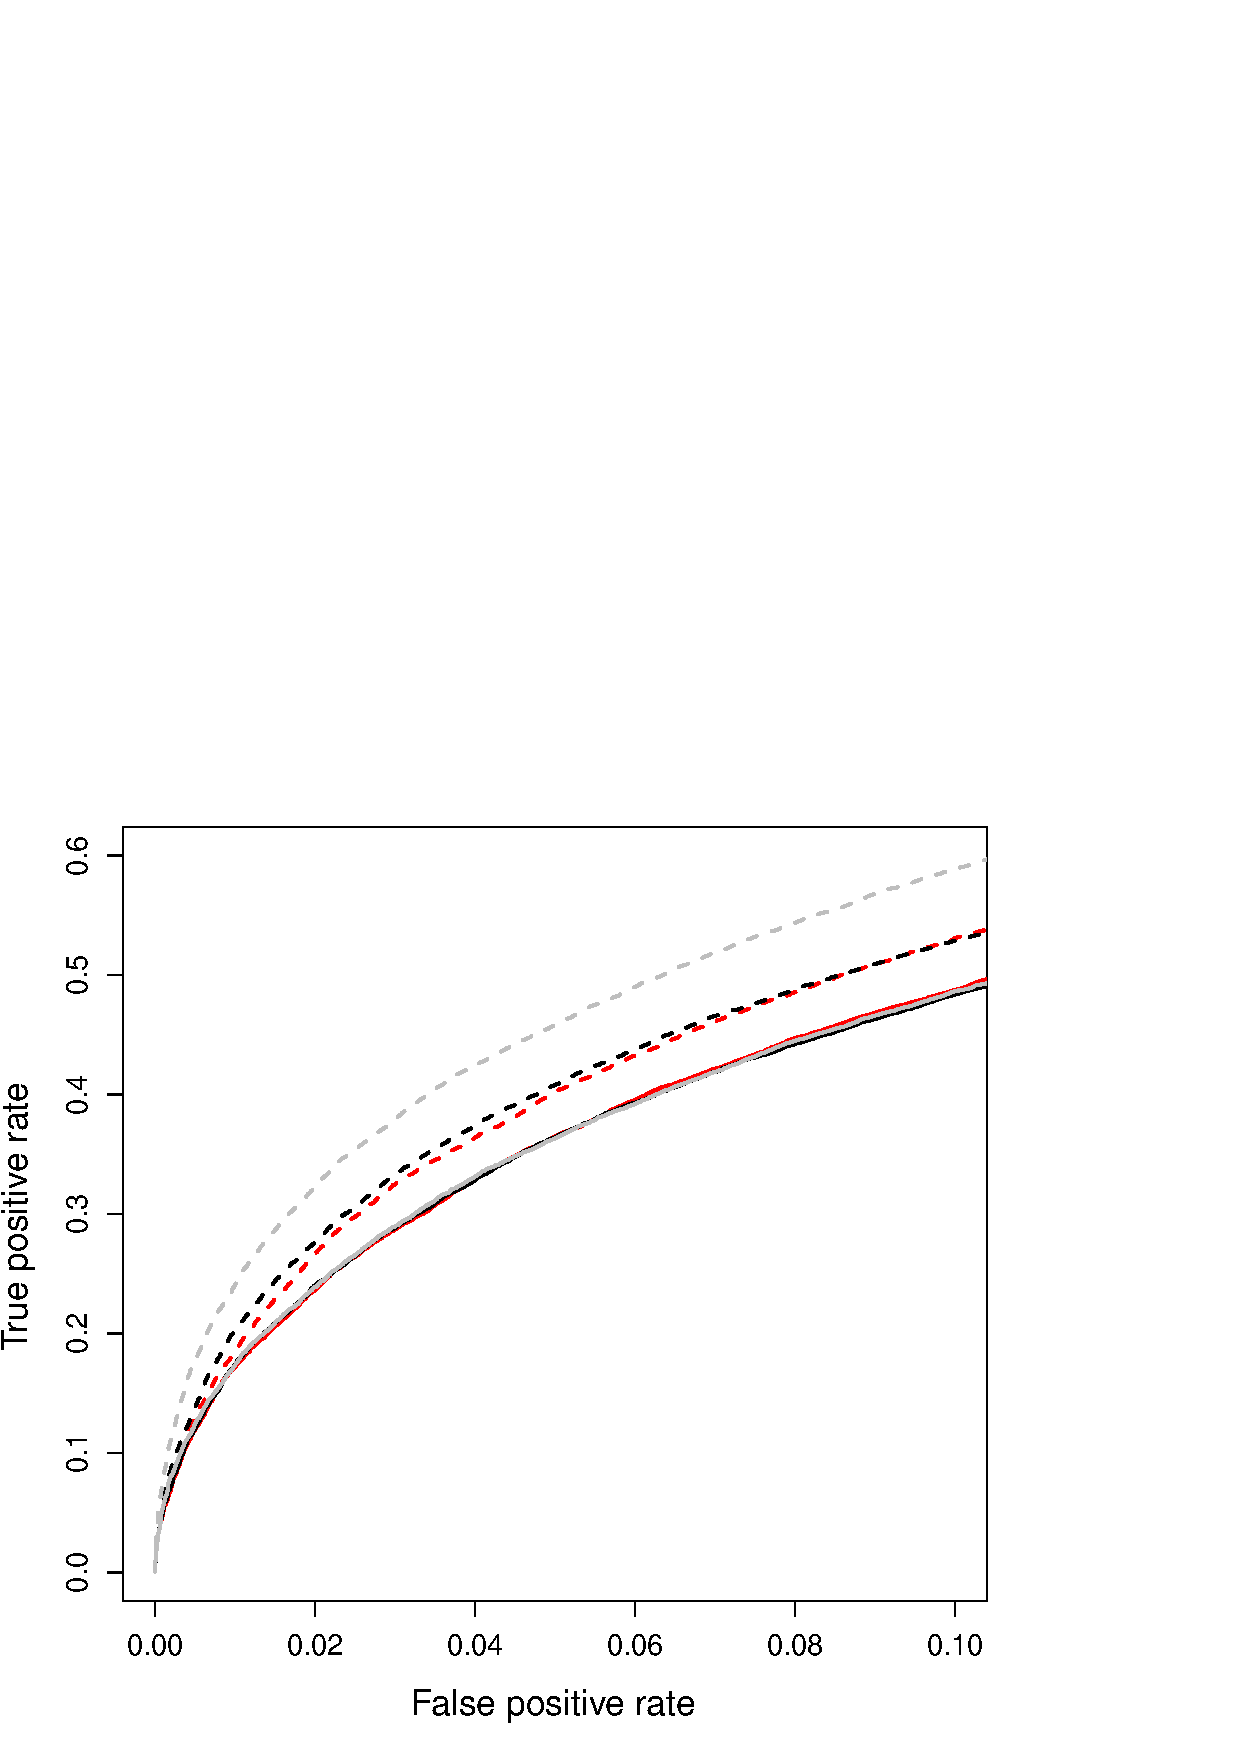
\includegraphics[width=0.48\textwidth]{power_with_zoom.pdf}
\end{center}
\caption{
    ROC curves for each analysis method on simulated data with a plate effect and genuine DE, for both single-cell (full) and summed counts (dashed).
    Curves are shown for DESeq2 (black), voom (grey) and edgeR (red).
    Each curve represents the average result of 10 simulation iterations.
    The full curves are shown on the left, and an enlarged plot focusing on low false positive rates is shown on the right.
}
\label{fig:roc}
\end{figure}

\begin{figure}[!p]
\begin{center}
\includegraphics[width=0.48\textwidth]{quantile_with.pdf}
%\includegraphics[width=0.48\textwidth,trim=0mm 0mm 0mm 10mm,clip]{quantile_without.pdf} % Doesn't really add any value; didn't put up control before either, so why do it now?
\end{center}
\caption{
    Observed type I error rates for QL edgeR on simulated data with a plate effect, 
        applied on counts from direct summation (black circles) or summation of quantile-adjusted pseudo-counts (grey diamonds). 
    Simulations were performed for a number of scenarios, including differing numbers of cells per plate (1);
        small (2), moderate (3) or large differences (4) in library size within plates;
        as well as the corresponding scenarios where replicate plates were swapped between groups.
    Error rates are shown on a log scale and represent the average of 10 simulation iterations.
    Each error bar represents the standard error of the corresponding log-average rate.
    The threshold of 0.01 is represented by the red dotted line.
}
\label{fig:complexplate}
\end{figure}

% Probably slightly more conservative than previous QL figure because n=2 here for each group, whereas n=3 before.

\begin{table}[!p]
\caption{Total number of DE genes detected by each method in each comparison at a FDR of 5\%, using the single-cell or summed counts.
The number of DE genes detected with both counts is also shown.
}
\label{tab:realnum}
\begin{center}
\begin{tabular}{l l r r r}
\hline
\textbf{Comparison} & \textbf{Counts} & \textbf{DESeq2} & \textbf{voom} & \textbf{edgeR} \\
\hline
\multirow{3}{*}{2i vs. serum} 
& Cell & 7419 & 9585 & 7127 \\
& Sum & 3227 & 1691 & 946 \\
& Shared & 2948 & 1678 & 946 \\
\hline
\multirow{3}{*}{a2i vs. serum} 
& Cell & 6447 & 9202 & 6013 \\
& Sum & 2004 & 758 & 238 \\
& Shared & 1876 & 747 & 238 \\
\hline
%\multirow{3}{*}{PS vs. NP} 
%& Cell & 268 & 4862 & 522 \\
%& Sum & 17 & 0 & 0 \\
%& Shared & 15 & 0 & 0 \\
%\hline
\end{tabular}
\end{center}
\end{table}

\begin{table}[!p]
\caption{Proportion of the top-ranking DE genes shared between analyses using the single-cell or summed counts.
Top genes were defined as those with the smallest 20, 200, or 2000 $p$-values in each comparison.
}
\label{tab:realrank}
\begin{center}
\begin{tabular}{l l r r r}
\hline
\textbf{Comparison} & \textbf{Top} & \textbf{DESeq2} & \textbf{voom} & \textbf{edgeR} \\
\hline
\multirow{3}{*}{2i vs. serum} 
& 20 & 0.10 & 0.05 & 0.20 \\
& 200 & 0.25 & 0.43 & 0.35 \\
& 2000 & 0.49 & 0.60 & 0.60 \\
\hline
\multirow{3}{*}{a2i vs. serum} 
& 20 & 0.30 & 0.15 & 0.20 \\
& 200 & 0.26 & 0.54 & 0.31 \\
& 2000 & 0.46 & 0.58 & 0.61 \\
\hline
%\multirow{3}{*}{PS vs. NP} 
%& 20 & 0.35 & 0.30 & 0.35 \\
%& 200 & 0.30 & 0.26 & 0.44 \\
%& 2000 & 0.39 & 0.26 & 0.66 \\
%\hline
\end{tabular}
\end{center}
\end{table}


\end{document}
